\chapter{Problema del corpo nero}

\section{Richiami su energia trasportata da onde}
\begin{definition}[Intensit\`a]
L'\textbf{intensit\`a} di un'onda \`e data da
\[I=\frac{dE}{dA_\perp dt}\qquad\qquad [I]=\frac{\mathrm{W}}{\mathrm{m}^{2}}.\]
La \textbf{radianza} \`e l'intensit\`a per angolo solido
\[I_\Omega=\frac{dE}{dA_\perp dtd\Omega}=\dd \Omega I.\]
\end{definition}

\begin{definition}[Emittanza e Irradianza]
L'\textbf{emittanza} come la potenza emessa da una supeficie per unit\`a di superficie. Si indica con $M$.\\
L'\textbf{irradianza} \`e la potenza ricevuta su una superficie per unit\`a di superficie. Anche questa si indica con $I$.
\end{definition}

\section{Pressione di radiazione}
Consideriamo un'onda elettromagnetica che incide su una superficie conduttrice in modo ortogonale. Sia $\sigma$ la densit\`a di carica superficiale. Se la superficie ha area $A$ allora possiamo scrivere la forza di Lorentz come
\[\frac{\vec F}A=\sigma(\vec E+\vec v\times \vec B).\]
L'onda induce un movimento delle cariche interno alla superficie e $\vec v\times \vec B$ ha verso sempre diretto verso la superficie

\begin{figure}[!htb]
    \centering
    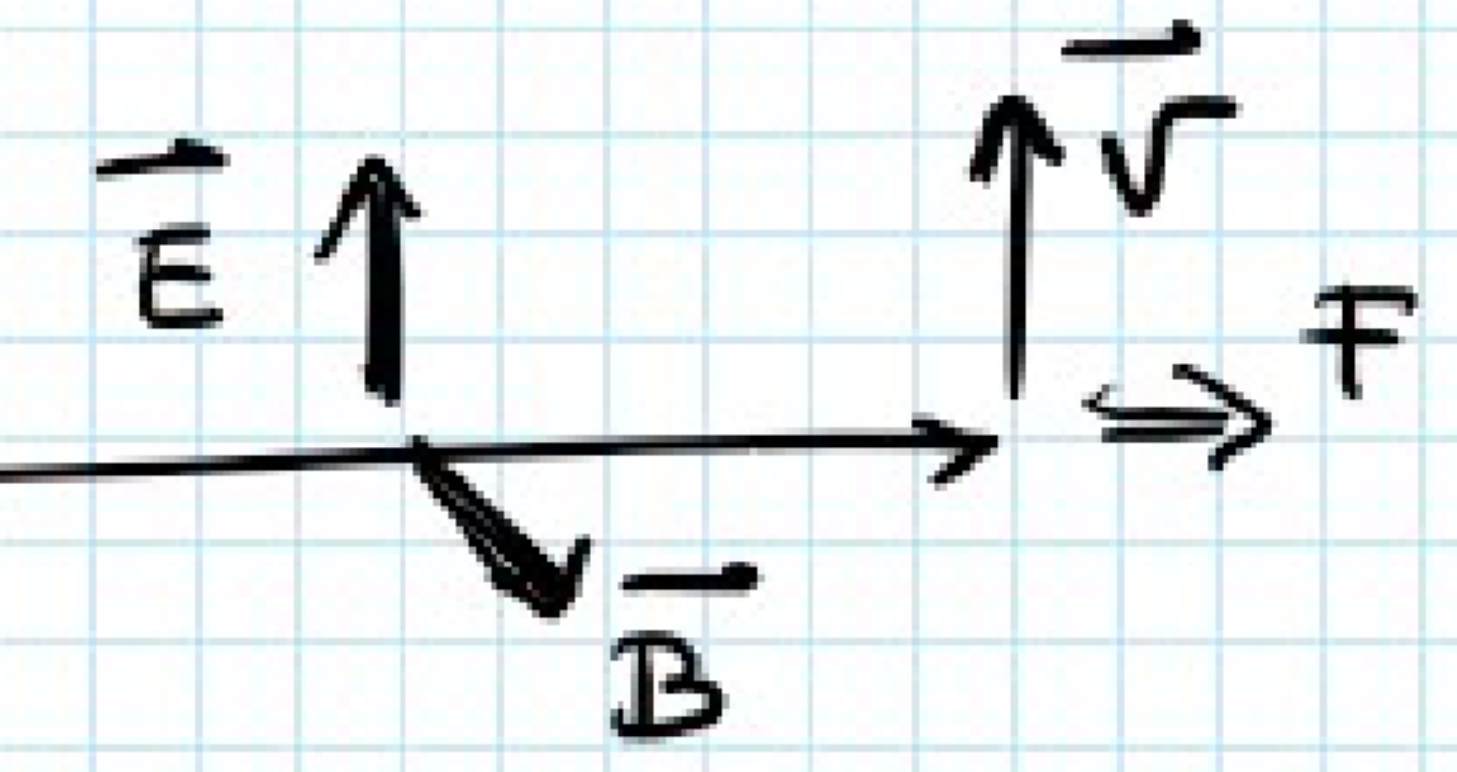
\includegraphics[width=5cm]{images/onda_elettromagnetica_che_incide_ortogonalmente.png}
\end{figure}

\noindent
Calcoliamo l'intensit\`a assorbita\footnote{potenza per area} e la pressione esercitata sulla superficie
\[\begin{cases}
~\\
I_{\text{assorbita}}=\dfrac{\vec F\cdot \vec v}A=\sigma \vec E\cdot \vec v+\cancelto{0}{\sigma \vec v\cdot(\vec v\times \vec B)}=\sigma \vec E\cdot \vec v\\\\
p\overset{\vec E\text{ parallelo}}{\overset{\text{a superficie}}=}\sigma\abs{\vec v\times \vec B}=\sigma vB=\sigma v\dfrac Ec=\dfrac{I_{\text{assorbita}}}c\\~
\end{cases}\]
Se la superficie assorbe tutta l'energia che riceve
\begin{align*}
&\Delta E=I_{\text{assorbita}}\Delta t A\\
&\abs{\vec p}=\frac1cI_{\text{assorbita}}\Delta t A
\end{align*}
Se la superficie riflette tutta l'energia che riceve
\begin{align*}
&\Delta E=0\\
&\abs{\vec p}=2\frac1cI_{\text{assorbita}}\Delta t A
\end{align*}

\subsection{Gas di onde elettromagnetiche}
Consideriamo una semisfera dentro la quale ci sono onde elettromagnetiche distribuite in modo omogeneo e isotropo. Sia $w$ la densit\`a di energia nella semisfera (ben definita per omogeneit\`a).\\
Consideriamo poi una superficie $A$ come in figura perfettamente assorbente e cerchiamo di capire quanta energia e quantit\`a di moto riceve per unit\`a di tempo.

\begin{figure}[!htb]
    \centering
    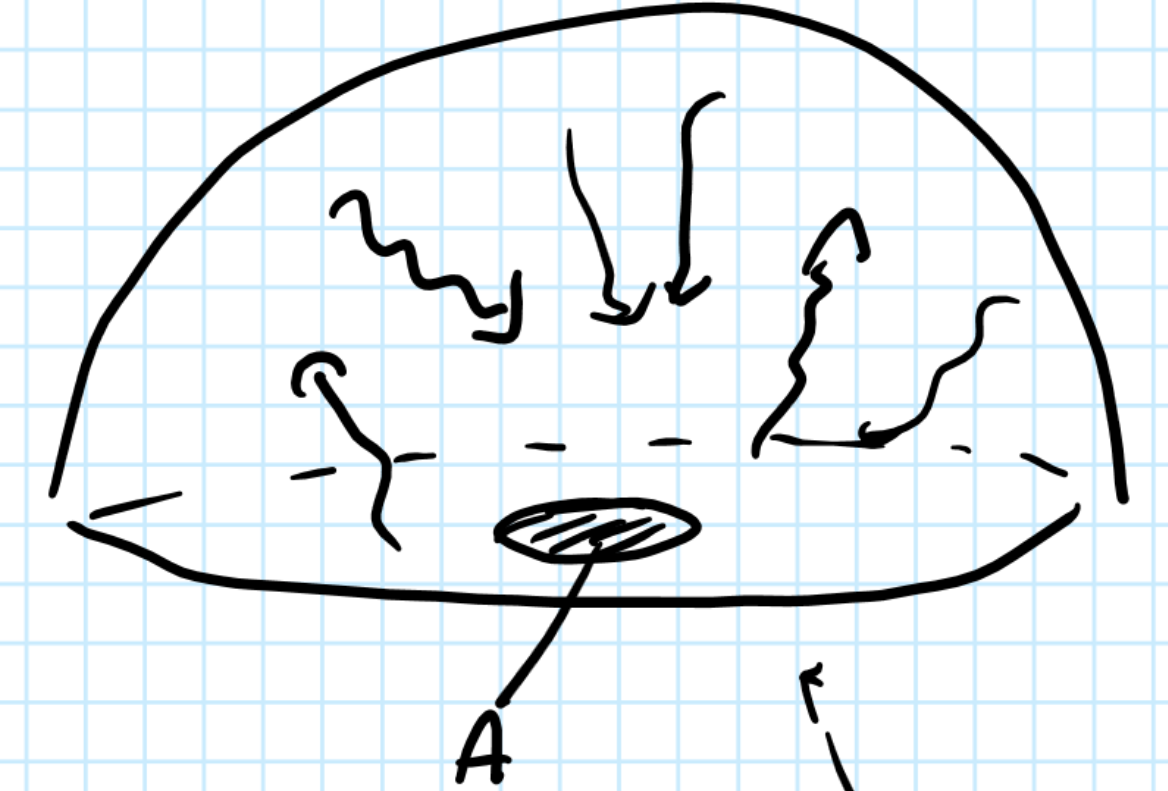
\includegraphics[width=5cm]{images/semisfera_luce.png}
\end{figure}

\noindent
Consideriamo un ragionamento analogo a quello fatto per il modello dei gas perfetti:\\
Fissata una direzione consideriamo il cilindro di particelle che si scontrano contro la nostra area in una unit\`a di tempo $dt$

\begin{figure}[!htb]
    \centering
    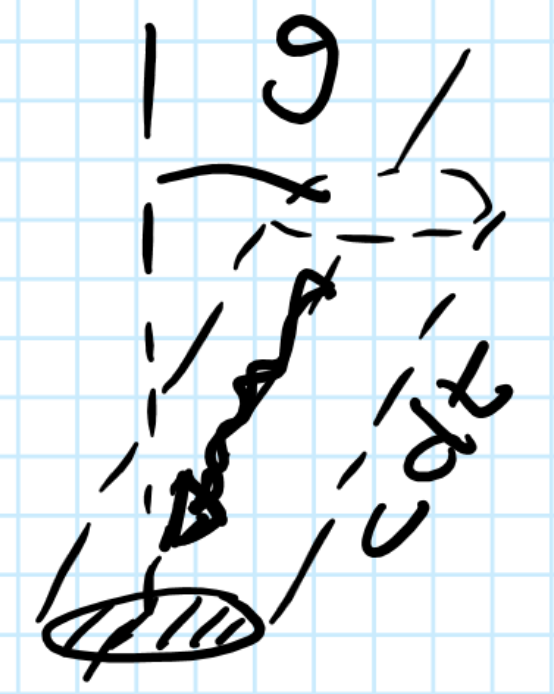
\includegraphics[width=2.5cm]{images/cilindretto_luce.png}
\end{figure}

\noindent
Il volume del cilindretto \`e $A cdt\cos \theta$, dunque l'energia che colpisce $A$ \`e
\[w Acdt\cos \theta.\]
Segue che tutta l'energia che raggiunge $A$ in un intervallo di tempo $dt$ \`e l'integrale sull'angolo solido diviso per due\footnote{stiamo considerando solo met\`a sfera} della quantit\`a trovata, cio\`e
\[dE=\frac12\int_\Omega w Acdt\cos\theta \frac{d\Omega}{4\pi}=\frac12\frac{w Acdt}{4\pi}\int_\Omega\cos\theta 2\pi \under{=d(\cos\theta)}{\sin\theta d\theta} =\frac{w cAdt}4,\]
dunque $I_{\text{assorbita}}=\dfrac{w c}4$.
\medskip

\noindent
Consideriamo ora l'impulso assorbito
\[d\abs{\vec p_\perp}\pasgnlmath={m_{\mathrm{luce}}=0}\frac{dE}c\cos\theta=\frac12\int_\Omega \frac w c Acdt(\cos\theta)^2 \frac{d\Omega}{4\pi}=\frac{w Adt}6,\]
dunque la pressione \`e
\[p=\frac w6.\]

\bigskip

\noindent
Se la superficie \`e riflettente allora $I_{\text{assorbita}}=0$ per definizione, quindi
\[d\abs{\vec p_\perp}=2\frac{w Adt}6\implies p=\frac w3.\]

\section{Radiazione di Corpo nero}
\subsection{Definizione e corpo nero scatola}
\begin{definition}[Assorbanza]
Un corpo irraggiato assorbe una frazione $a(\nu)$ della radiazione a frequenza $\nu$ che riceve. Questa quantit\`a \`e detta \textbf{assorbanza} (relativa alla frequenza $\nu$).
\end{definition}

\begin{definition}[Corpo bianco e corpo nero]
Se $a(\nu)=0$ per ogni $\nu$ allora il corpo \`e detto \textbf{bianco} o \textbf{perfettamente riflettente}.\\
Se $a(\nu)=1$ per ogni $\nu$ allora il corpo \`e detto \textbf{nero} o \textbf{perfettamente assorbente}.
\end{definition}

\begin{remark}
Poich\'e ogni oggetto contiene qualche particella carica, ogni corpo irraggia delle onde elettromagnetiche.
\end{remark}


\noindent
Una possibile realizzazione di un corpo nero \`e una scatola con pareti opache e un forellino minuscolo come in figura

\begin{figure}[!htb]
    \centering
    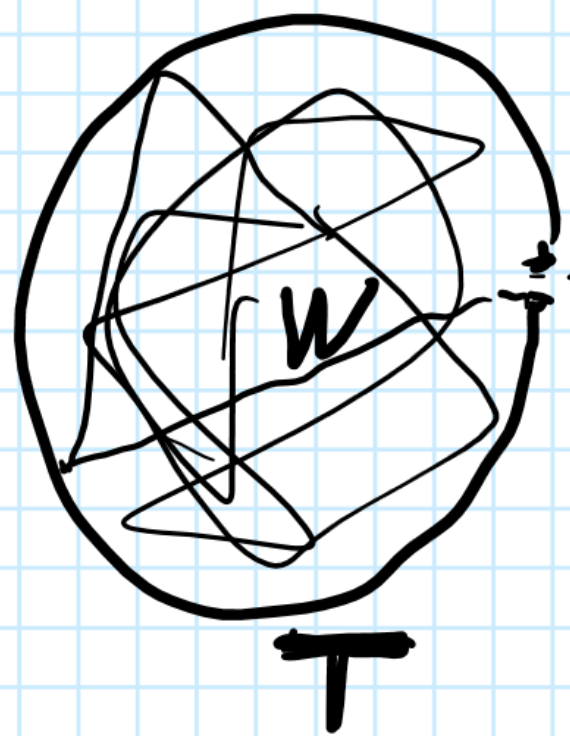
\includegraphics[width=2.5cm]{images/corpo_nero_scatola.png}
\end{figure}

\begin{proposition}
La densit\`a di energia di un corpo nero dipende solo da $T$. Inoltre la densit\`a di energia per ogni frequenza dipende solo da $T$.
\end{proposition}
\begin{proof}
Supponiamo di avere due corpi neri scatola, una con pareti interne perfettamente riflettenti e piene di energia e l'altra con pareti interne perfettamente assorbenti e poca energia.

\begin{figure}[!htb]
    \centering
    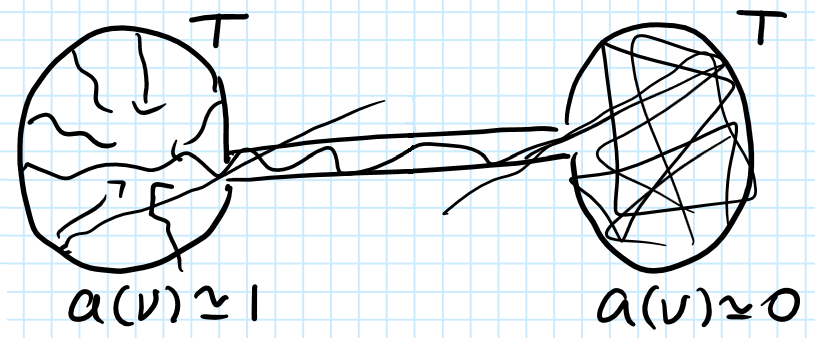
\includegraphics[width=7cm]{images/dimostrazione_w_dipende_solo_da_T.png}
\end{figure}

\noindent
Mettendo a contatto i forellini come in figura notiamo che le onde passerebbero dalla scatola riflettente a quella assorbente. Questo significa che anche se le sorgenti hanno la stessa temperatura, una tenderebbe a scaldarsi, negando il secondo principio.
\bigskip

\noindent
Se ora immaginiamo di mettere nel corridoio tra le scatole una parete che fa passare solo luce di una certa frequenza negeremmo di nuovo i principi della termodinamica se le densit\`a di energia fossero diverse per frequenze diverse.
\end{proof}

\subsection{Legge di Kirchhoff}
Immaginiamo ora di inserire un secondo corpo nero dentro la scatola. 
Per mantenere la sola dipendenza da $T$ si ha che per il corpo nero interno $I=M$, cio\`e assorbe tanta energia quanta ne emette.\\
Definiamo questa quantit\`a \textbf{radiazione di corpo nero}.

\begin{figure}[!htb]
    \centering
    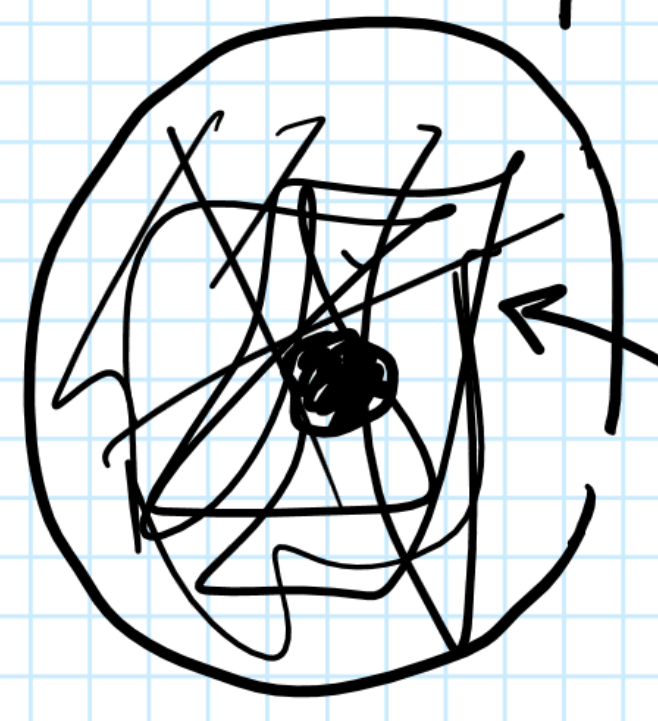
\includegraphics[width=2.5cm]{images/corpo_nero_con_dentro_corpo_nero.png}
\end{figure}

\noindent
Consideriamo ora lo steso scenario ma con un corpo non nero. Con un argomento analogo $aI=M$ in generale e per ogni frequenza $a(\nu)I_\nu=M_\nu$.

\begin{figure}[!htb]
    \centering
    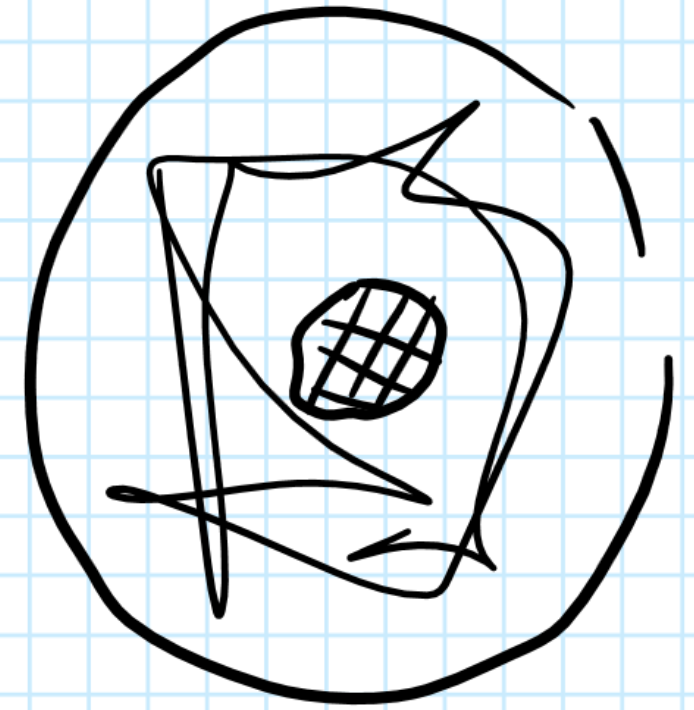
\includegraphics[width=2.5cm]{images/corpo_nero_con_dentro_corpo_grigio.png}
\end{figure}

\begin{remark}[Legge di Kirchhoff]
Il rapporto tra quanta radiazione un corpo emette rispetto ad un corpo nero alla stessa temperatura \`e esattamente la frazione di energia che assorbe
\[\frac{M}{M_{\text{corpo nero}}}=a.\]
Questa \`e la \textbf{legge di Kirchhoff}.
\end{remark}

\noindent Il ragionamento fatto funziona anche per frequenze fissate, quindi
\[\frac{M_\nu}{a(\nu)}=(M_\nu)_{\text{corpo nero}}.\]
Questo dimostra che la radiazione di corpo nero $(M_\nu)_{\text{corpo nero}}$ \`e una legge universale.

\subsection{Legge di Stefan-Boltzmann}
Osserviamo che
\[M=\int_0^\infty I_\nu d\nu=\frac{E_{\text{totale emessa}}}{\Delta t A}.\]
Sperimentalmente Stefan scopre che
\[M\propto T^4.\]
Boltzmann deduce questo risultato per via teorica:

\begin{theorem}[Legge di Stefan-Boltzmann]\label{LeggeStefanBoltzmann}
Vale la \textbf{legge di Stefan-Boltzmann}
\[M=\sigma T^4.\]
\end{theorem}
\begin{proof}
Modelliamo il corpo nero come una scatola con pareti interne perfettamente riflettenti.\\
Per definizione $w=\frac UV$, inoltre questo rapporto dipende solo da $T$.\\ Abbiamo calcolato prima che per pareti perfettamente riflettenti $p=\frac w3$, che dipende solo da $T$. Ricordando che per sistemi idrostatici $dU=TdS-pdV$, si ha che
\[dS=\frac {dU}T+\frac pTdV=\frac VTdw+\pa{\frac wT+\frac pT}dV.\]
Poich\'e $w$ dipende solo da $T$, se $T$ \`e costante allora $w$ \`e costante, quindi dalla relazione sopra segue che
\[s\doteqdot\ppb VST=\ppb VSw=\pa{\frac wT+\frac pT}=\frac 43 \frac wT,\]
dunque $S=sV$ e $s$ dipende solo da $T$.\\
Sviluppando di nuovo il primo principio si ha
\[wdV+Vdw=dU=TdS-pdV=TdS-\frac w3dV=T(sdV+Vds)-\frac w3dV.\]
Dividendo per $V$ troviamo
\[dw=Tds+\pa{Ts-\frac 43w}\frac{dV}V.\]
Portando $Tds$ al primo membro osserviamo che,
poich\'e $w$ e $s$ dipendono solo da $T$ (e in particolare non da $V$) entrambi i membri sono nulli, 
\[dw=Tds\quad\text{e}\quad Ts=\frac 43w.\]
Questo mostra che
\[\dd sw=T=\frac 43\frac ws\quad\pasgnl\implies{risolvi eq. diff.}\quad w\propto s^{4/3}\propto (w/T)^{4/3},\]
quindi $w\propto T^4$.
Segue che $M=I=\frac{wc}4\propto T^4$. Sia $\sigma$ la costante di proporzionalit\`a.
\end{proof}

\begin{fact}
La costante che appare nella legge di Stefan-Boltzmann, detta \textbf{costante di Stefan-Boltzmann} ha il valore
\[\sigma=5.67\cdot 10^{-8} \ \mathrm{W}\ \mathrm{m}^{-2}\ \mathrm{K}^{-4}.\]
\end{fact}